\documentclass[10pt,a4paper]{article}
\usepackage[pdftex]{graphicx}
\usepackage{graphicx}
\usepackage{amsmath}
\usepackage{listings}
\usepackage{url}
\usepackage{amsmath}
\usepackage[left=20mm, top=0in]{geometry}
\date{}
\begin{document}
\title{Assignment No 7}
\author{JAGAN M J EE20B047}
\maketitle


\section{AIM}

Aim is to analyse circuits using the Laplace Transform of the impulse response, utilsing the symbolic algebra capabilities of python

\section{Step response of a Low Pass Filter}
We aim to find the step response of the following circuit:

\begin{figure}[!tbh]

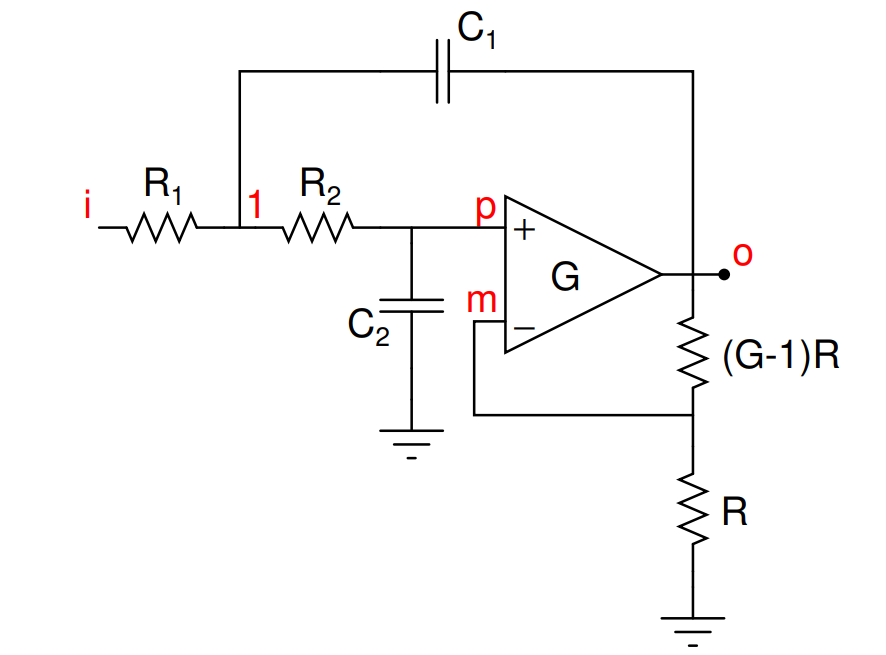
\includegraphics[width = 0.9\textwidth]{low pass filter circuit.png}
\caption{Low Pass Filter circuit}

\end{figure}

The output voltage Vo can be obtained in the s-domain using matrix capabilities of the Sympy module. For this the node voltages : \[ V1,  Vp,  Vm,  Vo \] can be obtained by solving the system of equations in the matrix form. After obtaining Vo, measures are written to convert its symbolic representation into its polynomial representaton compatible with the Signal toolbox of scipy: and following graph is obtained for step response :\\ \\ \\ \\ \\ \\ \\ \\ 

\begin{figure}[!tbh]

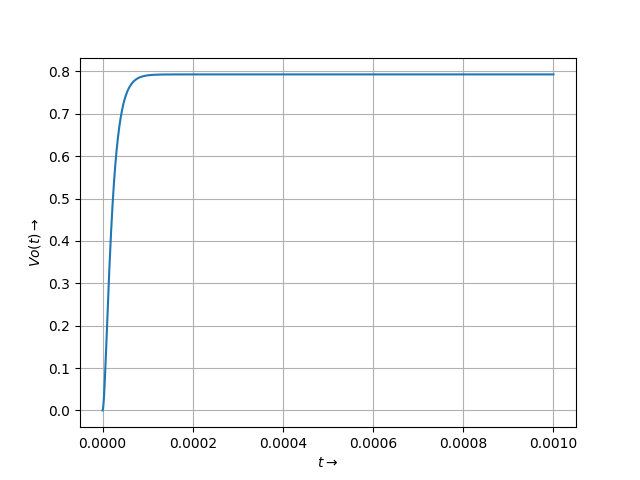
\includegraphics[width = 0.9\textwidth]{low pass filter step response.png}
\caption{Step Response of low pass filter}

\end{figure}

\section{Response for a mixed frequency input}

An input is applied which is in the form of : 

\begin{equation*}
  V_{i}(t) = ( \ \sin(2000\pi t) + \cos(2*10^{6}\pi t) \ )u_{o}(t) \ Volts
\end{equation*}

The following plot is obtained for the output voltage : \\ \\ \\ \\ \\ \\ \\ \\ \\ \\ \\ \\ \\ \\ \\ \\ \\ \\ \\ \\ \\ \\ \\ \\ \\ \\ 

\begin{figure}[!tbh]

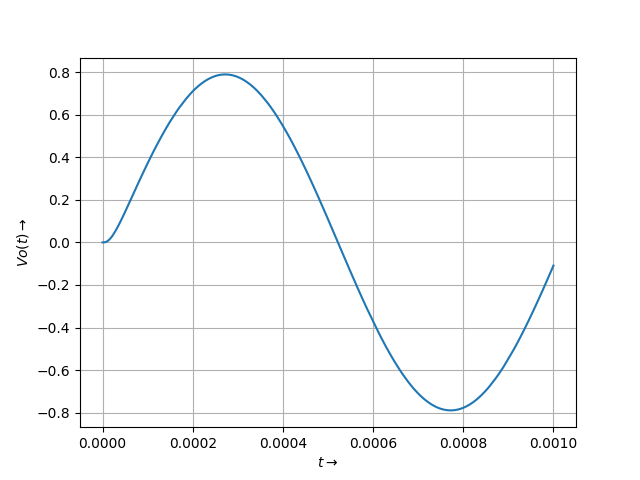
\includegraphics[width = 0.9\textwidth]{low pass filter Vo(t) for a Vi(t).png}
\caption{Output Voltage for low pass filter}

\end{figure}

Since the circuit is low pass filter, it is expected to pass through low frequency sine component and attenuates the high frequency cos component


\section{Magnitude Response of a High Pass Filter circuit}


We aim to find the magnitude response of the following circuit:

\begin{figure}[!tbh]

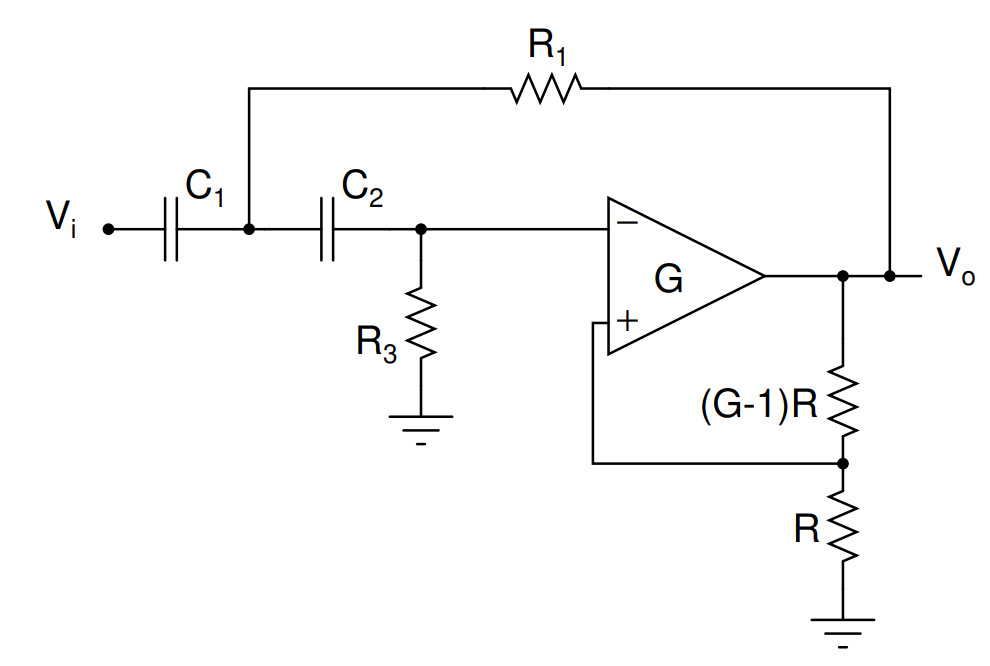
\includegraphics[width = 0.9\textwidth]{high pass filter circuit.png}
\caption{High Pass Filter circuit}

\end{figure}

The magnitude response of the High Pass filter circuit is as shown below:

\begin{figure}[!tbh]

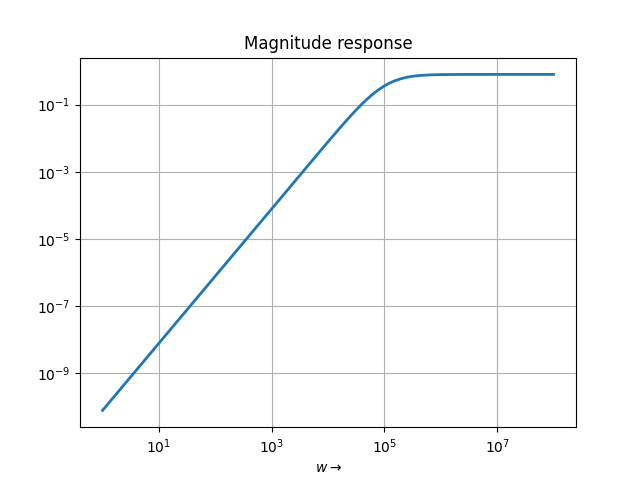
\includegraphics[width = 0.9\textwidth]{high pass filter magnitude response.png}
\caption{High Pass Filter circuit}

\end{figure}

\section{Response to a damped sinusoid}

Consider the following high frequency damped sinusoid :

\begin{equation*}
    V_{i}(t) = e^{-3000t}( \ \cos((10^7)t) \ ) Volts
\end{equation*}

\begin{figure}[!tbh]

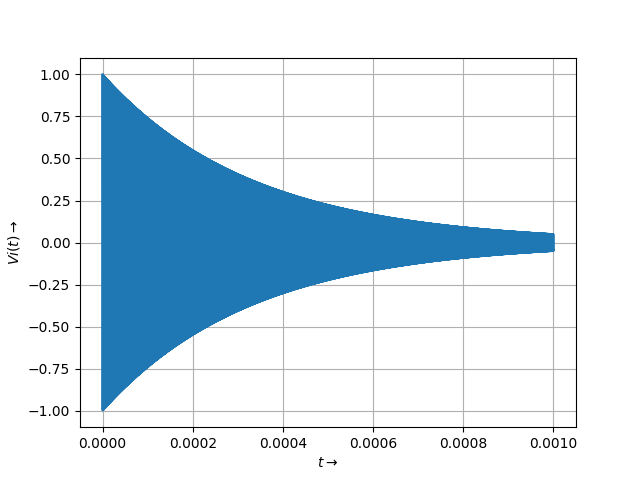
\includegraphics[width = 0.9\textwidth]{high frequency damped input.png}
\caption{Damped sinusoid}

\end{figure}

It is expected that the for a high pass filter, the input voltage will pass through with almost no change.\\ \\ \\ \\ \\ \\ \\ \\ \\ \\ \\ \\ \\ \\ \\ \\ \\ \\ \\ \\ \\

\begin{figure}[!tbh]

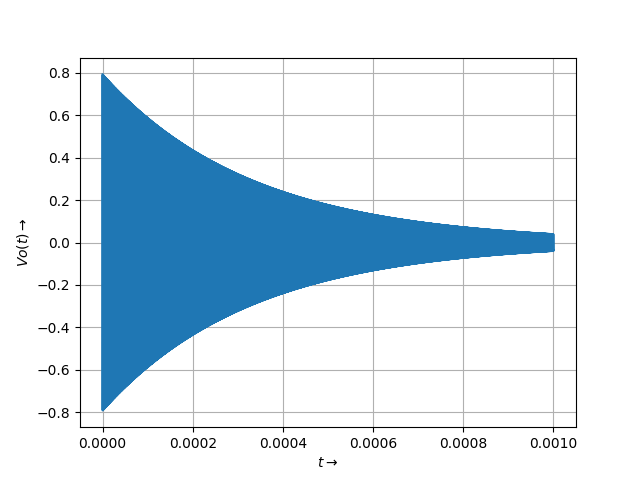
\includegraphics[width = 0.9\textwidth]{high pass filter Vo(t) for a damped Vi(t).png}
\caption{Damped response of a High Pass Filter}

\end{figure}


\section{Step response of a High Pass Filter}


As done in the case for low pass filter circuit, the following graph shows the step response of a high pass filter circuit : 

\begin{figure}[!tbh]

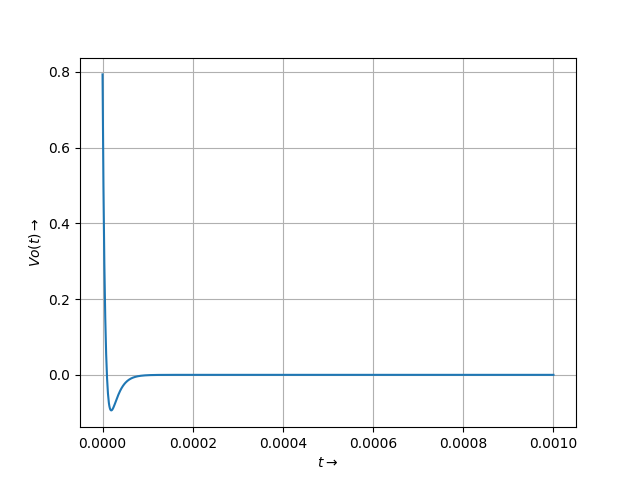
\includegraphics[width = 0.9\textwidth]{high pass filter step response.png}
\caption{Step Response of a high pass filter}

\end{figure}

\section{Conclusion}

Sympy provides a convenient way to analyse LTI systems using their Laplace transfroms. The toolbox was used to study the behaviour of a low pass filter, implemented using an opamp. For a mixed frequemcy sinusoid as input, it was found that the filter suppressed the high frequencies while allowing the low frequency components. Similarly, a high pass filter was implemented using an opamp . The magnitude response of this filter was plotted and its output was analysed for damped sinusoids. The step response of this filter was also plotted and was found to have a non zero peak at beginning, due to sudden change in the input voltage

\end{document}